%%
%% This is file `squelette-rr.tex',
%% generated with the docstrip utility.
%%
%% The original source files were:

%%
%% RR.dtx  (with options: `sample')
%% ********************************************************************
%% Copyright (C) 1997-1999 2004 2006 2007 INRIA/APICS by Jose' Grimm
%% This file may be distributed and/or modified under the
%% conditions of the LaTeX Project Public License, either version 1.3
%% of this license or (at your option) any later version.
%% The latest version of this license is in
%%    http://www.latex-project.org/lppl.txt
%% and version 1.3 or later is part of all distributions of LaTeX
%% version 2003/12/01 or later.
%% An archive of the software can be found at
%%    ftp://ftp-sop.inria.fr/apics/rr-inria

\documentclass[a4paper]{article}

\usepackage{RR}
%\usepackage{hyperref}
\usepackage{a4wide}
%\usepackage{comment}
%\excludecomment{figure}
%%\usepackage[frenchb]{babel} % optionnel
%%
%% date de publication du rapport
\RRdate{\today}
%%
%% Cas d'une version deux
%% \RRversion{2}
%% date de publication de la version 2
%% \RRdater{Novembre  2006}

%%
\RRauthor{% % les auteurs
%  % Premier auteur, avec une note
% Vincent Acary\thanks{\tt vincent.acary@inrialpes.fr}%
%   % note partag\'ee (optionnelle)
% %  \thanks[sfn]{Shared foot note}%
%  \and Maurice Br\'emond\thanks{\tt maurice.bremond@inrialpes.fr}
% %entre chaque auteur s'il y en a plusieurs
%   \and
% Florent Cadoux\thanks{florent.cadoux@gmail.com}%
%  % r\'ef\'erence \`a la note partag\'ee
% %\thanksref{sfn}
}
%%
%% Ceci apparait sur chaque page paire.
\authorhead{}
%%
\RRtitle{Sur la r\'esolution du probl\`eme de frottement tridimensionnel. Formulations and comparaisons des m\'ethodes num\'eriques. }
%% English title
\RRetitle{Solving 3D frictional contact problems: Formulations and comparisons of numerical methods.}
%%
\titlehead{Solving 3D frictional contact problems}
%%
%\RRnote{}
%\RRnote{This is a second note}
%%
\RRresume{TBW
}
\RRabstract{TBW}
%%
\RRmotcle{Syst\`emes multi--corps, M\'ecanique non r\'eguli\`ere, contraintes unilat\'erales,  frottement de Coulomb, impact, Sch\'emas num\'eriques de r\'esolution}
\RRkeyword{ Multibody systems, nonsmooth Mechanics,  unilateral constraints, Coulomb friction, impact, numerical methods}
%%
%% \Rrprojet{Apics}  % cas d'un seul projet
\RRprojet{Bipop}
%%
%%\RRtheme{\THNum} % cas d'un seul theme
%%\RRtheme{\THCom \THCog \THSym \THNum \THBio} % cas de 5 themes
%%
%% \URLorraine % pour ceux qui sont \`a l'est
%% \URRennes  % pour ceux qui sont \`a l'ouest
 \URRhoneAlpes % pour ceux qui sont dans les montagnes
%% \URRocq % pour ceux qui sont au centre de la France
%% \URFuturs % pour ceux qui sont dans le virtuel
%% \URSophia % pour ceux qui sont au Sud.
%%
%% \RCBordeaux % centre de recherche Bordeaux - Sud Ouest
%% \RCLille % centre de recherche Lille Nord Europe
%% \RCParis % Paris Rocquencourt
%% \RCSaclay % Saclay \^Ile de France
\RCGrenoble % Grenoble - Rh\^one-Alpes
%% \RCNancy % Nancy - Grand Est
%% \RCRennes % Rennes - Bretagne Atlantique
%\RCSophia % Sophia Antipolis M\'editerran\'ee


\usepackage{geometry}
\usepackage{layout}
\geometry{
  left=2.5cm,
  right=2.5cm,
  top=3.5cm,
  bottom=3cm
}

\usepackage{natbib}
% For unicode 
%\usepackage{ucs}
\usepackage[utf8]{inputenc}
%\usepackage[utf8]{inputenc}
\usepackage[T1]{fontenc}
\usepackage[english]{babel}

% invisible unicode space
\DeclareUnicodeCharacter{00A0}{~}

\usepackage{mathtools, amsthm, amssymb}

\usepackage{graphicx}
\usepackage{psfrag}

%\usepackage{subfigure}
\usepackage{subfig,float}
\usepackage{rotating}

% table package
\usepackage{hhline}
\usepackage{multicol} % for column
\usepackage{tabularx} % for beautiful column

% math packages 
\usepackage{amsmath,amsthm,amsfonts,amssymb,amsbsy,stmaryrd} 

\usepackage{subeqnarray}



% pour la cesure des mots
%\usepackage[T1]{fontenc}
%\usepackage{inputenc}
\usepackage{textcomp}

%pour l'environnement remarque
%\usepackage{theorem}
%\usepackage{ntheorem}

%pour faire des symboles d\'ebiles
\usepackage{pifont}
%pour faire des minis tables des matieres

\usepackage{algorithm}
\usepackage{algorithmic}

%\usepackage[numbers]{natbib}

\renewcommand{\cite}[1]{\protect\citep{#1}}
%\def\cite#1{\citep{#1}}
%\usepackage{draftcopy}

\usepackage{float}
%\usepackage{showkeys}
\usepackage{showlabels}

\usepackage{array}



\usepackage{tikz}
\usepackage{xkeyval,tkz-base}
\usetikzlibrary{arrows}
\usetikzlibrary{calc}

\usepackage{fancyhdr}
\usepackage{lastpage}


\usepackage[pdfencoding=unicode,pdftex,backref=page]{hyperref}






../../../TeX/Report/macro.tex

%\newcommand{\includegraphicsmaybe}[1]{\IfFileExists{{#1}}{\includegraphics{#1}}{\makebox{‌​File {#1} is missing}}}

\fancyfoot[L]{}
\fancyfoot[C]{}
\fancyfoot[R]{\texttt{file rr.tex -- \isodayandtime}}

\newcommand{\test}[4]{
\section{{#2} precision {#3} timeout {#4}}
\begin{figure}[htbp]
  \centering
  \includegraphics[width=\figwidth]{../figure/VI/UpdateRule/{#3}/{#4}/\measurename/profile-#1.pdf}
  \includegraphics[width=\figwidth]{../figure/VI/UpdateRule/{#3}/{#4}/\measurename/profile-#1_legend.pdf}
\caption{{#2}{  } \measurename{  } VI/UpdateRule}
\end{figure}

\begin{figure}[htbp]
  \centering
  \includegraphics[width=\figwidth]{../figure/NSGS/LocalSolver/{#3}/{#4}/\measurename/profile-#1.pdf}
  \includegraphics[width=\figwidth]{../figure/NSGS/LocalSolver/{#3}/{#4}/\measurename/profile-#1_legend.pdf}
\caption{{#2}{  } \measurename { }NSGS/LocalSolver}
\end{figure}

\begin{figure}[htbp]
  \centering
  \includegraphics[width=\figwidth]{../figure/NSGS/LocalSolverHybrid/{#3}/{#4}/\measurename/profile-#1.pdf}
  \includegraphics[width=\figwidth]{../figure/NSGS/LocalSolverHybrid/{#3}/{#4}/\measurename/profile-#1_legend.pdf}
\caption{{#2}{  } \measurename { }NSGS/LocalSolverHybrid}
\end{figure}

\begin{figure}[htbp]
  \centering
  \includegraphics[width=\figwidth]{../figure/NSGS/LocalTol/{#3}/{#4}/\measurename/profile-#1.pdf}
  \includegraphics[width=\figwidth]{../figure/NSGS/LocalTol/{#3}/{#4}/\measurename/profile-#1_legend.pdf}
\caption{{#2}{  } \measurename { }NSGS/LocalTol}
\end{figure}

\begin{figure}[htbp]
  \centering
  \includegraphics[width=\figwidth]{../figure/NSGS/LocalTol/VI/{#3}/{#4}/\measurename/profile-#1.pdf}
  \includegraphics[width=\figwidth]{../figure/NSGS/LocalTol/VI/{#3}/{#4}/\measurename/profile-#1_legend.pdf}
\caption{{#2}{  } \measurename { }NSGS/LocalTol-VI}
\end{figure}

\begin{figure}[htbp]
  \centering
  \includegraphics[width=\figwidth]{../figure/NSGS/Shuffled/{#3}/{#4}/\measurename/profile-#1.pdf}
  \includegraphics[width=\figwidth]{../figure/NSGS/Shuffled/{#3}/{#4}/\measurename/profile-#1_legend.pdf}
\caption{{#2}{  } \measurename { }NSGS/Shuffled}
\end{figure}

\begin{figure}[htbp]
  \centering
  \includegraphics[width=\figwidth]{../figure/PSOR/{#3}/{#4}/\measurename/profile-#1.pdf}
  \includegraphics[width=\figwidth]{../figure/PSOR/{#3}/{#4}/\measurename/profile-#1_legend.pdf}
\caption{{#2}{  } \measurename { }PSOR}
\end{figure}

\begin{figure}[htbp]
  \centering
  \includegraphics[width=\figwidth]{../figure/NSN/{#3}/{#4}/\measurename/profile-#1.pdf}
  \includegraphics[width=\figwidth]{../figure/NSN/{#3}/{#4}/\measurename/profile-#1_legend.pdf}
\caption{{#2}{  } \measurename { }NSN}
\end{figure}

\begin{figure}[htbp]
  \centering
  \includegraphics[width=\figwidth]{../figure/PROX/InternalSolvers/{#3}/{#4}/\measurename/profile-#1.pdf}
  \includegraphics[width=\figwidth]{../figure/PROX/InternalSolvers/{#3}/{#4}/\measurename/profile-#1_legend.pdf}
\caption{{#2}{  } \measurename { }PROX/InternalSolvers}
\end{figure}

\begin{figure}[htbp]
  \centering
  \includegraphics[width=\figwidth]{../figure/PROX/Parameters/nu05/{#3}/{#4}/\measurename/profile-#1.pdf}
  \includegraphics[width=\figwidth]{../figure/PROX/Parameters/nu05/{#3}/{#4}/\measurename/profile-#1_legend.pdf}
\caption{{#2}{  } \measurename { }PROX/Parametric studies $\nu=0.5$}
\end{figure}

\begin{figure}[htbp]
  \centering
  \includegraphics[width=\figwidth]{../figure/PROX/Parameters/nu10/{#3}/{#4}/\measurename/profile-#1.pdf}
  \includegraphics[width=\figwidth]{../figure/PROX/Parameters/nu10/{#3}/{#4}/\measurename/profile-#1_legend.pdf}
\caption{{#2}{  } \measurename { }PROX/Parametric studies $\nu=1.0$}
\end{figure}

\begin{figure}[htbp]
  \centering
  \includegraphics[width=\figwidth]{../figure/PROX/Parameters/nu20/{#3}/{#4}/\measurename/profile-#1.pdf}
  \includegraphics[width=\figwidth]{../figure/PROX/Parameters/nu20/{#3}/{#4}/\measurename/profile-#1_legend.pdf}
\caption{{#2}{  } \measurename { }PROX/Parametric studies $\nu=2.0$}
\end{figure}

\begin{figure}[htbp]
  \centering
  \includegraphics[width=\figwidth]{../figure/REGUL/{#3}/{#4}/\measurename/profile-#1.pdf}
  \includegraphics[width=\figwidth]{../figure/REGUL/{#3}/{#4}/\measurename/profile-#1_legend.pdf}
\caption{{#2}{  } \measurename { }PROX/Regularized problem}
\end{figure}


\begin{figure}[htbp]
  \centering
  \includegraphics[width=\figwidth]{../figure/OPTI/{#3}/{#4}/\measurename/profile-#1.pdf}
  \includegraphics[width=\figwidth]{../figure/OPTI/{#3}/{#4}/\measurename/profile-#1_legend.pdf}
\caption{{#2}{  } \measurename { }OPTI}
\end{figure}


\begin{figure}[htbp]
  \centering
  \includegraphics[width=\figwidth]{../figure/COMP/large/{#3}/{#4}/\measurename/profile-#1.pdf}
  \includegraphics[width=\figwidth]{../figure/COMP/large/{#3}/{#4}/\measurename/profile-#1_legend.pdf}
\caption{{#2}{  } \measurename { }COMP/large}
\end{figure}


\begin{figure}[htbp]
  \centering
  \includegraphics[width=\figwidth]{../figure/COMP/zoom/{#3}/{#4}/\measurename/profile-#1.pdf}
  \includegraphics[width=\figwidth]{../figure/COMP/zoom/{#3}/{#4}/\measurename/profile-#1_legend.pdf}
\caption{{#2}{  } \measurename { }COMP/zoom}
\end{figure}

}



\begingroup
\count0=\time \divide\count0by60 % Hour
\count2=\count0 \multiply\count2by-60 \advance\count2by\time
% Min
\def\2#1{\ifnum#1<10 0\fi\the#1}
\xdef\isodayandtime{\the\year-\2\month-\2\day\space\2{\count0}:%
\2{\count2}}
\endgroup
%%%% fin macro %%%%

\graphicspath{{../figure/}}

\PassOptionsToPackage{dvipsnames,svgnames}{xcolor}
\renewcommand{\baselinestretch}{1.5}
\usepackage{natbib}
%%
\begin{document}
%%
\RRNo{123456789}
\makeRR   % cas d'un rapport de recherche
%% \makeRT % cas d'un rapport technique.
%% a partir d'ici, chacun fait comme il le souhaite



\tableofcontents

\def\figwidth{0.33\textwidth}
\def\legendwidth{0.6\textwidth}
\def\legendheight{0.15\textheight}
\def\subfiglayout{%
  \captionsetup[subfloat]{farskip=-0pt,captionskip=-2pt,font=scriptsize}%
  \setlength{\abovecaptionskip}{0pt}}



\section{Numerical methods for VI: {\sf FP-DS, FP-VI-$\star$} and {\sf FP-EG-$\star$}}
\label{Sec:Comparison,VI,step-length}

\begin{figure*}[htbp]
  \centering
  \subfiglayout
\subfloat[\scriptsize LowWall\_FEM]
   {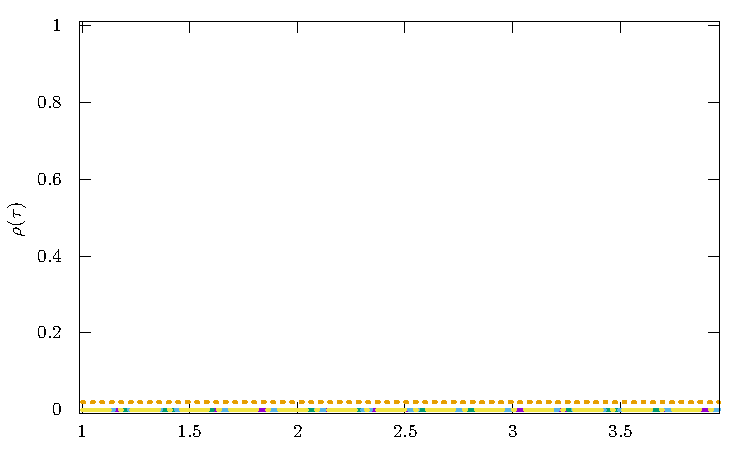
\includegraphics[width=\figwidth]{../figure/VI/UpdateRule/1.0e-04/400/time/profile-LMGC_LowWall_FEM.pdf}} 
\subfloat[\scriptsize Cubes\_H8 II]
   {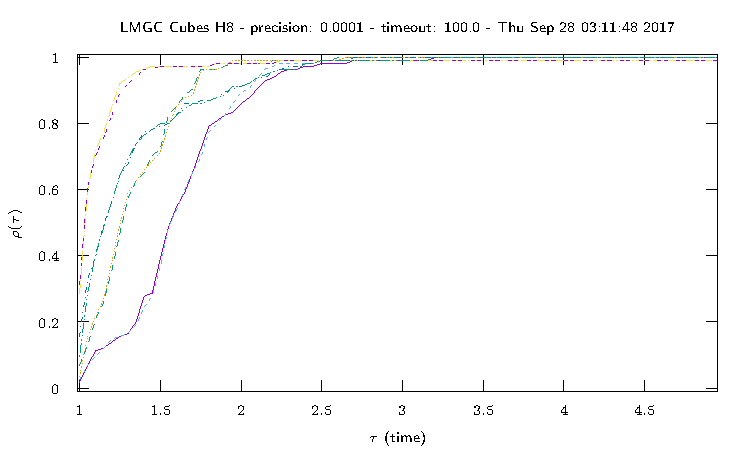
\includegraphics[width=\figwidth]{../figure/VI/UpdateRule/1.0e-04/100/time/profile-LMGC_Cubes_H8.pdf}} 
\subfloat[\scriptsize Cubes\_H8]
   {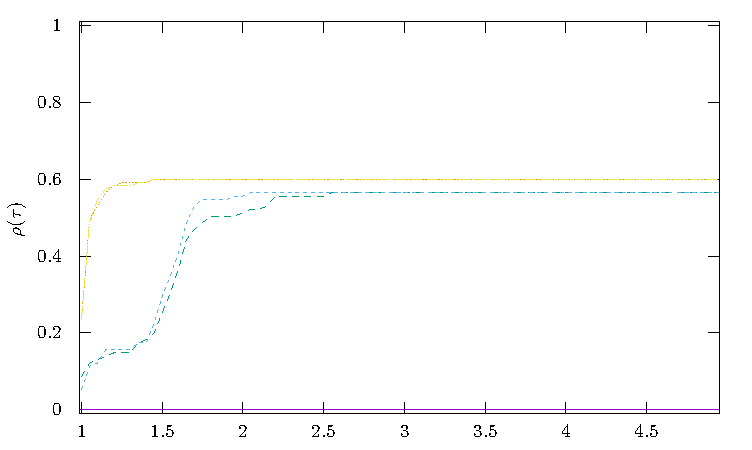
\includegraphics[width=\figwidth]{../figure/VI/UpdateRule/1.0e-08/100/time/profile-LMGC_Cubes_H8.pdf}} \\
\subfloat[\scriptsize Bridge\_PR II]
   {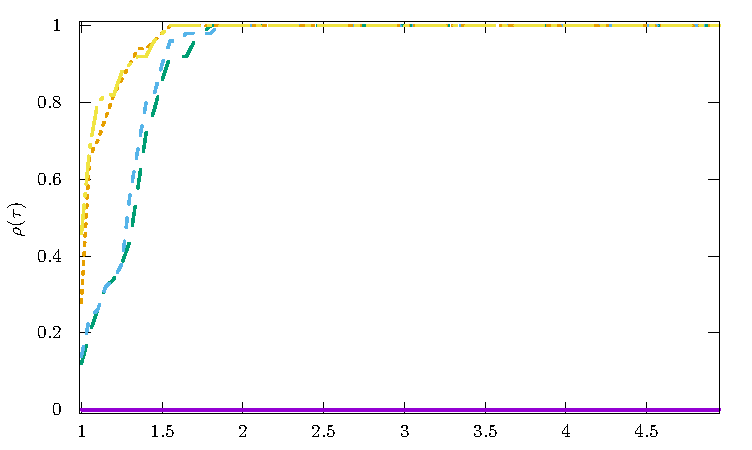
\includegraphics[width=\figwidth]{../figure/VI/UpdateRule/1.0e-04/100/time/profile-LMGC_Bridge_PR.pdf}} 
\subfloat[\scriptsize Bridge\_PR]
   {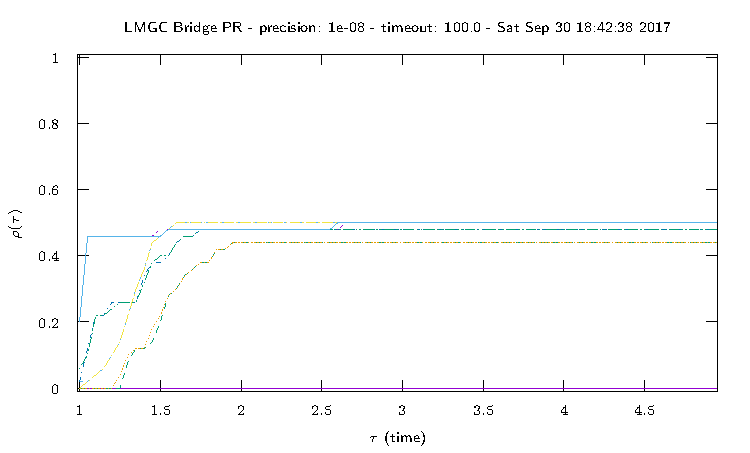
\includegraphics[width=\figwidth]{../figure/VI/UpdateRule/1.0e-08/100/time/profile-LMGC_Bridge_PR.pdf}} 
\subfloat[\scriptsize AqueducPR]
   {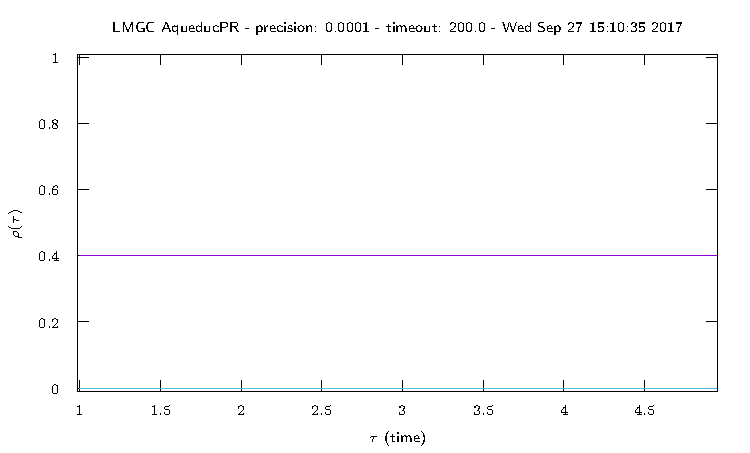
\includegraphics[width=\figwidth]{../figure/VI/UpdateRule/1.0e-04/200/time/profile-LMGC_AqueducPR.pdf}} \\
\subfloat[\scriptsize 945\_SP\_Box\_PL]
   {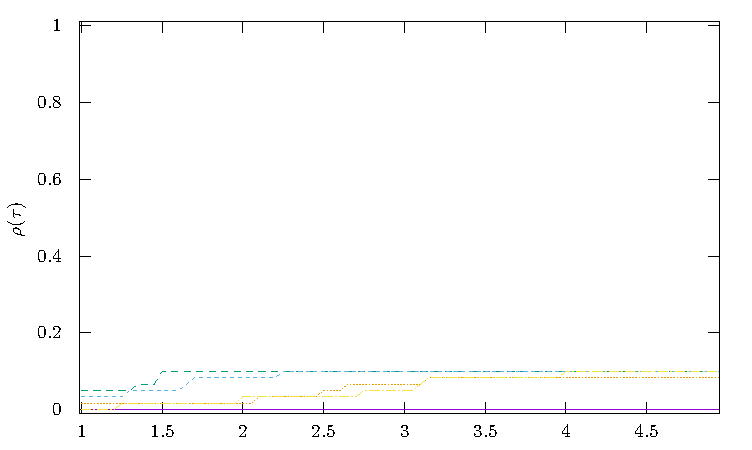
\includegraphics[width=\figwidth]{../figure/VI/UpdateRule/1.0e-04/100/time/profile-LMGC_945_SP_Box_PL.pdf}} 
\subfloat[\scriptsize 100\_PR\_PerioBox II]
   {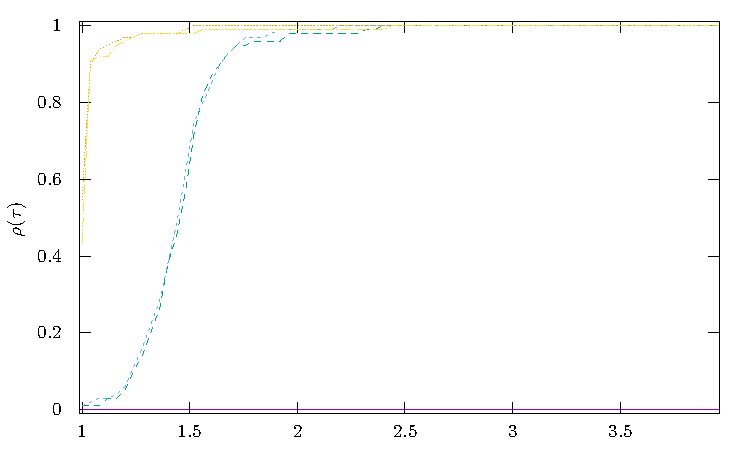
\includegraphics[width=\figwidth]{../figure/VI/UpdateRule/1.0e-04/100/time/profile-LMGC_100_PR_PerioBox.pdf}} 
\subfloat[\scriptsize 100\_PR\_PerioBox]
   {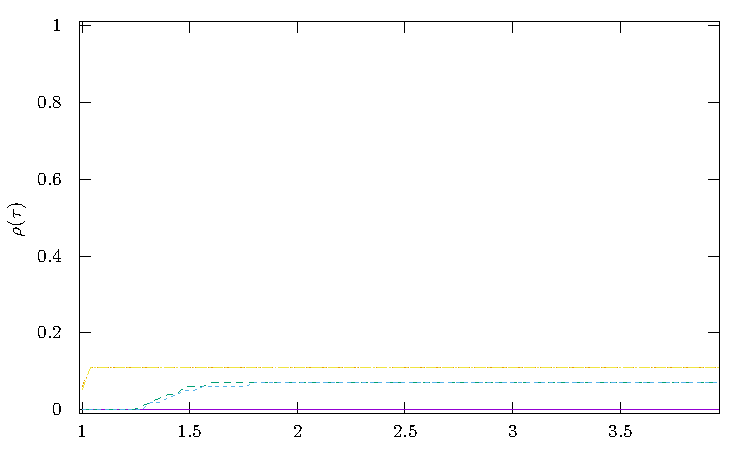
\includegraphics[width=\figwidth]{../figure/VI/UpdateRule/1.0e-08/200/time/profile-LMGC_100_PR_PerioBox.pdf}} \\
\subfloat[\scriptsize KaplasTower II]
   {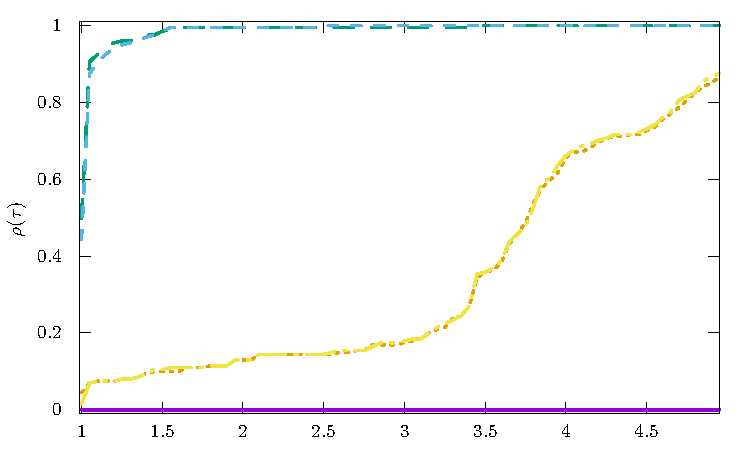
\includegraphics[width=\figwidth]{../figure/VI/UpdateRule/1.0e-04/100/time/profile-KaplasTower.pdf}} 
\subfloat[\scriptsize KaplasTower]
   {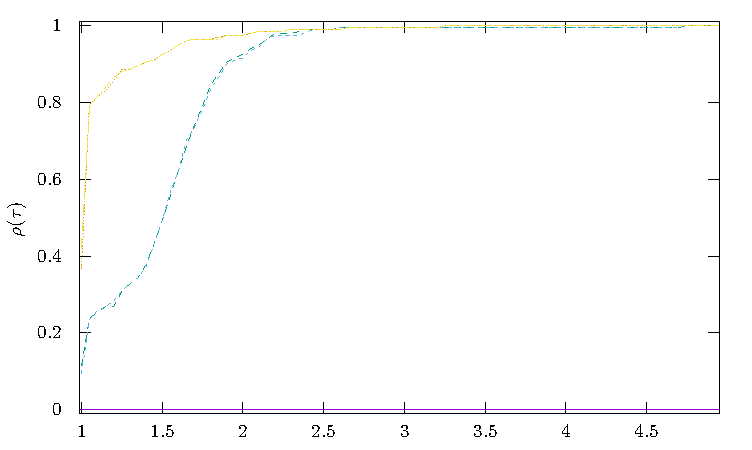
\includegraphics[width=\figwidth]{../figure/VI/UpdateRule/1.0e-08/200/time/profile-KaplasTower.pdf}} 
\subfloat[\scriptsize Chute\_local\_problems II]
   {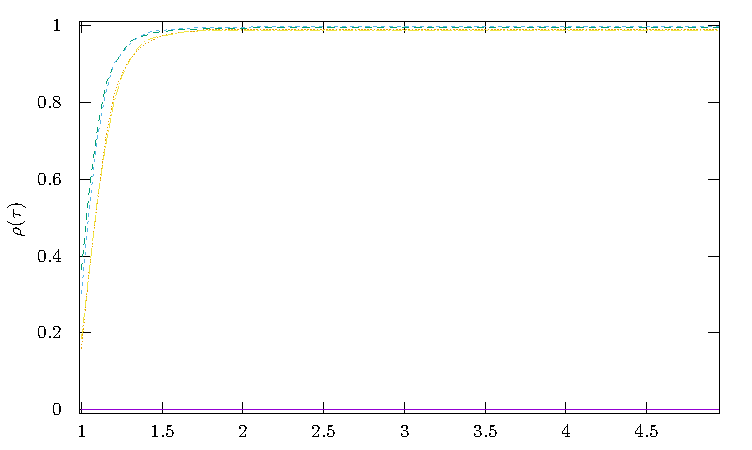
\includegraphics[width=\figwidth]{../figure/VI/UpdateRule/1.0e-04/10/time/profile-Chute_local_problems.pdf}} \\
\subfloat[\scriptsize Chute\_local\_problems]
   {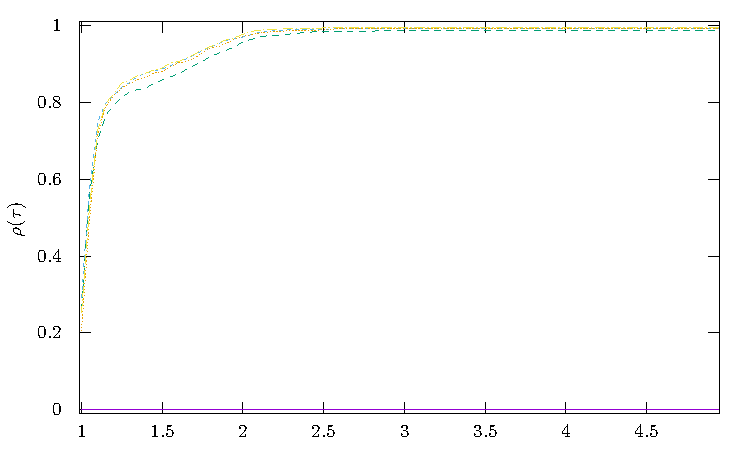
\includegraphics[width=\figwidth]{../figure/VI/UpdateRule/1.0e-08/10/time/profile-Chute_local_problems.pdf}} 
\subfloat[\scriptsize Chute\_4000]
   {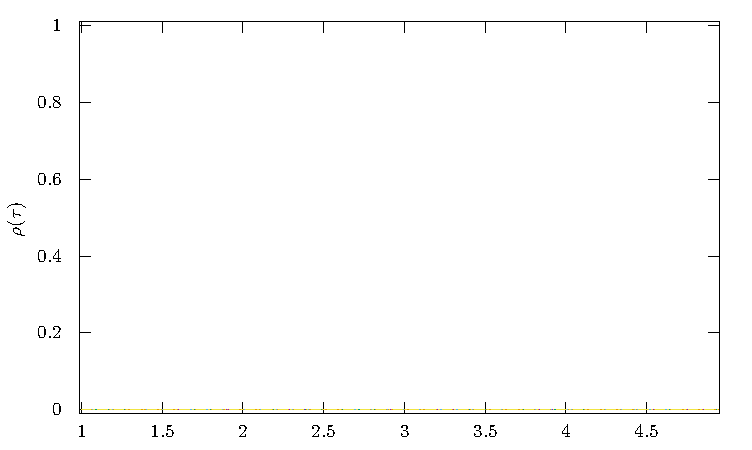
\includegraphics[width=\figwidth]{../figure/VI/UpdateRule/1.0e-04/200/time/profile-Chute_4000.pdf}} 
\subfloat[\scriptsize Chute\_1000]
   {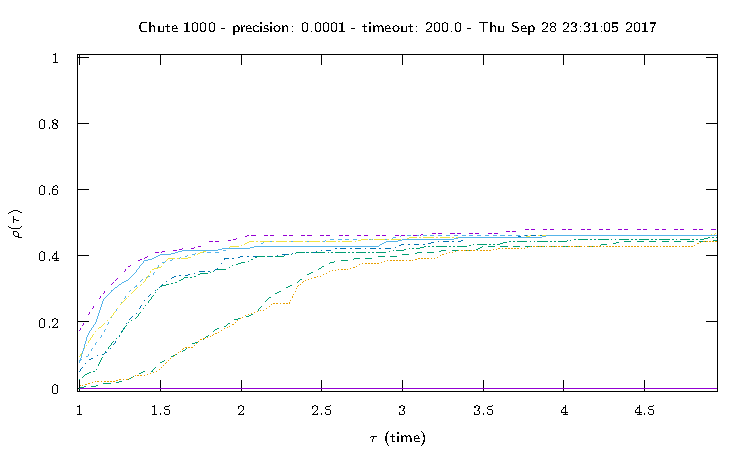
\includegraphics[width=\figwidth]{../figure/VI/UpdateRule/1.0e-04/200/time/profile-Chute_1000.pdf}} \\
\subfloat[\scriptsize Chain]
   {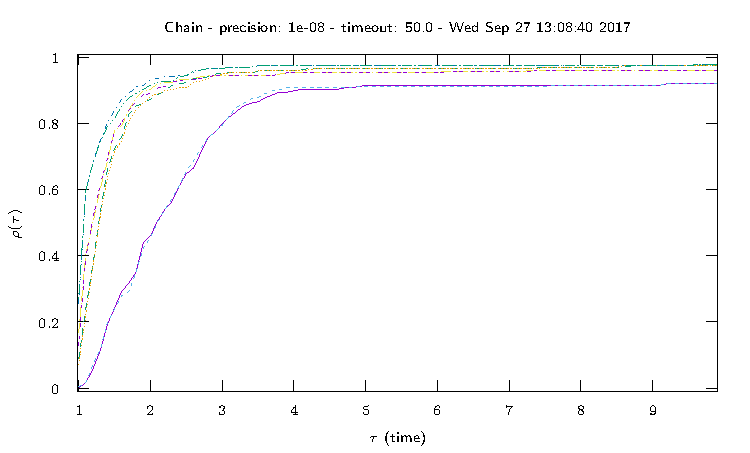
\includegraphics[width=\figwidth]{../figure/VI/UpdateRule/1.0e-08/50/time/profile-Chain.pdf}} 
\subfloat[\scriptsize Capsules]
   {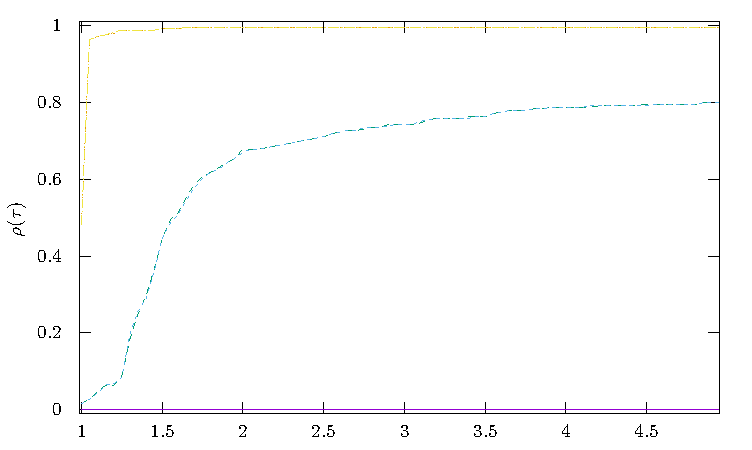
\includegraphics[width=\figwidth]{../figure/VI/UpdateRule/1.0e-08/50/time/profile-Capsules.pdf}} 
\subfloat[\scriptsize BoxesStack]
   {\includegraphics[width=\figwidth]{../figure/VI/UpdateRule/1.0e-08/100/time/profile-BoxesStack1.pdf}} \\
{\includegraphics[height=\legendheight]{../figure/VI/UpdateRule/1.0e-08/50/time/profile-Chain_legend.pdf}} 
   \caption{Comparison of numerical method for VI  {\sf FP-DS, FP-VI-$\star$} and {\sf FP-EG-$\star$}}
\label{fig:VI/UpdateRule}
\end{figure*}

\section{Splitting based algorithms: {\sf NSGS-$\star$} and {\sf PSOR-$\star$}}


\begin{figure}
  \centering
    \subfiglayout
\subfloat[\scriptsize LowWall\_FEM]
   {\includegraphics[width=\figwidth]{../figure/NSGS/LocalSolver/1.0e-04/400/time/profile-LMGC_LowWall_FEM.pdf}} 
\subfloat[\scriptsize Cubes\_H8 II]
   {\includegraphics[width=\figwidth]{../figure/NSGS/LocalSolver/1.0e-04/100/time/profile-LMGC_Cubes_H8.pdf}} 
\subfloat[\scriptsize Cubes\_H8]
   {\includegraphics[width=\figwidth]{../figure/NSGS/LocalSolver/1.0e-08/100/time/profile-LMGC_Cubes_H8.pdf}} \\
\subfloat[\scriptsize Bridge\_PR II]
   {\includegraphics[width=\figwidth]{../figure/NSGS/LocalSolver/1.0e-04/100/time/profile-LMGC_Bridge_PR.pdf}} 
\subfloat[\scriptsize Bridge\_PR]
   {\includegraphics[width=\figwidth]{../figure/NSGS/LocalSolver/1.0e-08/100/time/profile-LMGC_Bridge_PR.pdf}} 
\subfloat[\scriptsize AqueducPR]
   {\includegraphics[width=\figwidth]{../figure/NSGS/LocalSolver/1.0e-04/200/time/profile-LMGC_AqueducPR.pdf}} \\
\subfloat[\scriptsize 945\_SP\_Box\_PL]
   {\includegraphics[width=\figwidth]{../figure/NSGS/LocalSolver/1.0e-04/100/time/profile-LMGC_945_SP_Box_PL.pdf}} 
\subfloat[\scriptsize 100\_PR\_PerioBox II]
   {\includegraphics[width=\figwidth]{../figure/NSGS/LocalSolver/1.0e-04/100/time/profile-LMGC_100_PR_PerioBox.pdf}} 
\subfloat[\scriptsize 100\_PR\_PerioBox]
   {\includegraphics[width=\figwidth]{../figure/NSGS/LocalSolver/1.0e-08/200/time/profile-LMGC_100_PR_PerioBox.pdf}} \\
\subfloat[\scriptsize KaplasTower II]
   {\includegraphics[width=\figwidth]{../figure/NSGS/LocalSolver/1.0e-04/100/time/profile-KaplasTower.pdf}} 
\subfloat[\scriptsize KaplasTower]
   {\includegraphics[width=\figwidth]{../figure/NSGS/LocalSolver/1.0e-08/200/time/profile-KaplasTower.pdf}} 
\subfloat[\scriptsize Chute\_local\_problems II]
   {\includegraphics[width=\figwidth]{../figure/NSGS/LocalSolver/1.0e-04/10/time/profile-Chute_local_problems.pdf}} \\
\subfloat[\scriptsize Chute\_local\_problems]
   {\includegraphics[width=\figwidth]{../figure/NSGS/LocalSolver/1.0e-08/10/time/profile-Chute_local_problems.pdf}} 
\subfloat[\scriptsize Chute\_4000]
   {\includegraphics[width=\figwidth]{../figure/NSGS/LocalSolver/1.0e-04/200/time/profile-Chute_4000.pdf}} 
\subfloat[\scriptsize Chute\_1000]
   {\includegraphics[width=\figwidth]{../figure/NSGS/LocalSolver/1.0e-04/200/time/profile-Chute_1000.pdf}} \\
\subfloat[\scriptsize Chain]
   {\includegraphics[width=\figwidth]{../figure/NSGS/LocalSolver/1.0e-08/50/time/profile-Chain.pdf}} 
\subfloat[\scriptsize Capsules]
   {\includegraphics[width=\figwidth]{../figure/NSGS/LocalSolver/1.0e-08/50/time/profile-Capsules.pdf}} 
\subfloat[\scriptsize BoxesStack]
   {\includegraphics[width=\figwidth]{../figure/NSGS/LocalSolver/1.0e-08/100/time/profile-BoxesStack1.pdf}} \\
{\includegraphics[height=\legendheight]{../figure/NSGS/LocalSolver/1.0e-08/50/time/profile-Chain_legend.pdf}} 
  \caption{Influence of the local solver in {\sf NSGS-$\star$} algorithms.}
  \label{fig:NSGS/LocalSolver}
\end{figure}



\paragraph{Influence of the tolerance of the local solver $\sf tol_{local}$ in {\sf NSGS-FP-VI-UPK} algorithms}

\begin{figure}
  \centering
    \subfiglayout
\subfloat[\scriptsize LowWall\_FEM]
   {\includegraphics[width=\figwidth]{../figure/NSGS/LocalTol/VI/1.0e-04/400/time/profile-LMGC_LowWall_FEM.pdf}} 
\subfloat[\scriptsize Cubes\_H8 II]
   {\includegraphics[width=\figwidth]{../figure/NSGS/LocalTol/VI/1.0e-04/100/time/profile-LMGC_Cubes_H8.pdf}} 
\subfloat[\scriptsize Cubes\_H8]
   {\includegraphics[width=\figwidth]{../figure/NSGS/LocalTol/VI/1.0e-08/100/time/profile-LMGC_Cubes_H8.pdf}} \\
\subfloat[\scriptsize Bridge\_PR II]
   {\includegraphics[width=\figwidth]{../figure/NSGS/LocalTol/VI/1.0e-04/100/time/profile-LMGC_Bridge_PR.pdf}} 
\subfloat[\scriptsize Bridge\_PR]
   {\includegraphics[width=\figwidth]{../figure/NSGS/LocalTol/VI/1.0e-08/100/time/profile-LMGC_Bridge_PR.pdf}} 
\subfloat[\scriptsize AqueducPR]
   {\includegraphics[width=\figwidth]{../figure/NSGS/LocalTol/VI/1.0e-04/200/time/profile-LMGC_AqueducPR.pdf}} \\
\subfloat[\scriptsize 945\_SP\_Box\_PL]
   {\includegraphics[width=\figwidth]{../figure/NSGS/LocalTol/VI/1.0e-04/100/time/profile-LMGC_945_SP_Box_PL.pdf}} 
\subfloat[\scriptsize 100\_PR\_PerioBox II]
   {\includegraphics[width=\figwidth]{../figure/NSGS/LocalTol/VI/1.0e-04/100/time/profile-LMGC_100_PR_PerioBox.pdf}} 
\subfloat[\scriptsize 100\_PR\_PerioBox]
   {\includegraphics[width=\figwidth]{../figure/NSGS/LocalTol/VI/1.0e-08/200/time/profile-LMGC_100_PR_PerioBox.pdf}} \\
\subfloat[\scriptsize KaplasTower II]
   {\includegraphics[width=\figwidth]{../figure/NSGS/LocalTol/VI/1.0e-04/100/time/profile-KaplasTower.pdf}} 
\subfloat[\scriptsize KaplasTower]
   {\includegraphics[width=\figwidth]{../figure/NSGS/LocalTol/VI/1.0e-08/200/time/profile-KaplasTower.pdf}} 
\subfloat[\scriptsize Chute\_local\_problems II]
   {\includegraphics[width=\figwidth]{../figure/NSGS/LocalTol/VI/1.0e-04/10/time/profile-Chute_local_problems.pdf}} \\
\subfloat[\scriptsize Chute\_local\_problems]
   {\includegraphics[width=\figwidth]{../figure/NSGS/LocalTol/VI/1.0e-08/10/time/profile-Chute_local_problems.pdf}} 
\subfloat[\scriptsize Chute\_4000]
   {\includegraphics[width=\figwidth]{../figure/NSGS/LocalTol/VI/1.0e-04/200/time/profile-Chute_4000.pdf}} 
\subfloat[\scriptsize Chute\_1000]
   {\includegraphics[width=\figwidth]{../figure/NSGS/LocalTol/VI/1.0e-04/200/time/profile-Chute_1000.pdf}} \\
\subfloat[\scriptsize Chain]
   {\includegraphics[width=\figwidth]{../figure/NSGS/LocalTol/VI/1.0e-08/50/time/profile-Chain.pdf}} 
\subfloat[\scriptsize Capsules]
   {\includegraphics[width=\figwidth]{../figure/NSGS/LocalTol/VI/1.0e-08/50/time/profile-Capsules.pdf}} 
\subfloat[\scriptsize BoxesStack]
   {\includegraphics[width=\figwidth]{../figure/NSGS/LocalTol/VI/1.0e-08/100/time/profile-BoxesStack1.pdf}} \\
{\includegraphics[height=\legendheight]{../figure/NSGS/LocalTol/VI/1.0e-08/50/time/profile-Chain_legend.pdf}} 
\caption{Influence of the tolerance of the local solver $\sf tol_{local}$ in {\sf NSGS-FP-VI-UPK} algorithms.}
 \label{fig:NSGS/LocalTol/VI}
\end{figure}

\paragraph{Influence of the tolerance of the local solver $\sf tol_{local}$ in {\sf NSGS-AC-GP} algorithms.}




\begin{figure}
  \centering
    \subfiglayout
\subfloat[\scriptsize LowWall\_FEM]
   {\includegraphics[width=\figwidth]{../figure/NSGS/LocalTol/1.0e-04/400/time/profile-LMGC_LowWall_FEM.pdf}} 
\subfloat[\scriptsize Cubes\_H8 II]
   {\includegraphics[width=\figwidth]{../figure/NSGS/LocalTol/1.0e-04/100/time/profile-LMGC_Cubes_H8.pdf}} 
\subfloat[\scriptsize Cubes\_H8]
   {\includegraphics[width=\figwidth]{../figure/NSGS/LocalTol/1.0e-08/100/time/profile-LMGC_Cubes_H8.pdf}} \\
\subfloat[\scriptsize Bridge\_PR II]
   {\includegraphics[width=\figwidth]{../figure/NSGS/LocalTol/1.0e-04/100/time/profile-LMGC_Bridge_PR.pdf}} 
\subfloat[\scriptsize Bridge\_PR]
   {\includegraphics[width=\figwidth]{../figure/NSGS/LocalTol/1.0e-08/100/time/profile-LMGC_Bridge_PR.pdf}} 
\subfloat[\scriptsize AqueducPR]
   {\includegraphics[width=\figwidth]{../figure/NSGS/LocalTol/1.0e-04/200/time/profile-LMGC_AqueducPR.pdf}} \\
\subfloat[\scriptsize 945\_SP\_Box\_PL]
   {\includegraphics[width=\figwidth]{../figure/NSGS/LocalTol/1.0e-04/100/time/profile-LMGC_945_SP_Box_PL.pdf}} 
\subfloat[\scriptsize 100\_PR\_PerioBox II]
   {\includegraphics[width=\figwidth]{../figure/NSGS/LocalTol/1.0e-04/100/time/profile-LMGC_100_PR_PerioBox.pdf}} 
\subfloat[\scriptsize 100\_PR\_PerioBox]
   {\includegraphics[width=\figwidth]{../figure/NSGS/LocalTol/1.0e-08/200/time/profile-LMGC_100_PR_PerioBox.pdf}} \\
\subfloat[\scriptsize KaplasTower II]
   {\includegraphics[width=\figwidth]{../figure/NSGS/LocalTol/1.0e-04/100/time/profile-KaplasTower.pdf}} 
\subfloat[\scriptsize KaplasTower]
   {\includegraphics[width=\figwidth]{../figure/NSGS/LocalTol/1.0e-08/200/time/profile-KaplasTower.pdf}} 
\subfloat[\scriptsize Chute\_local\_problems II]
   {\includegraphics[width=\figwidth]{../figure/NSGS/LocalTol/1.0e-04/10/time/profile-Chute_local_problems.pdf}} \\
\subfloat[\scriptsize Chute\_local\_problems]
   {\includegraphics[width=\figwidth]{../figure/NSGS/LocalTol/1.0e-08/10/time/profile-Chute_local_problems.pdf}} 
\subfloat[\scriptsize Chute\_4000]
   {\includegraphics[width=\figwidth]{../figure/NSGS/LocalTol/1.0e-04/200/time/profile-Chute_4000.pdf}} 
\subfloat[\scriptsize Chute\_1000]
   {\includegraphics[width=\figwidth]{../figure/NSGS/LocalTol/1.0e-04/200/time/profile-Chute_1000.pdf}} \\
\subfloat[\scriptsize Chain]
   {\includegraphics[width=\figwidth]{../figure/NSGS/LocalTol/1.0e-08/50/time/profile-Chain.pdf}} 
\subfloat[\scriptsize Capsules]
   {\includegraphics[width=\figwidth]{../figure/NSGS/LocalTol/1.0e-08/50/time/profile-Capsules.pdf}} 
\subfloat[\scriptsize BoxesStack]
   {\includegraphics[width=\figwidth]{../figure/NSGS/LocalTol/1.0e-08/100/time/profile-BoxesStack1.pdf}} \\
{\includegraphics[height=\legendheight]{../figure/NSGS/LocalTol/1.0e-08/50/time/profile-Chain_legend.pdf}}  
\caption{Influence of the tolerance of the local solver $\sf tol_{local}$ in {\sf NSGS-FP-NSN-AC-GP} algorithms.}
\label{fig:NSGS/LocalTol}
\end{figure}


\paragraph{Influence of the choice of the parameters $\rho_\n, \rho_\t$ in the local solver of the {\sf NSGS-AC} algorithms}
\begin{figure}
  \centering
    \subfiglayout
\subfloat[\scriptsize LowWall\_FEM]
   {\includegraphics[width=\figwidth]{../figure/NSGS/rho/1.0e-04/400/time/profile-LMGC_LowWall_FEM.pdf}} 
\subfloat[\scriptsize Cubes\_H8 II]
   {\includegraphics[width=\figwidth]{../figure/NSGS/rho/1.0e-04/100/time/profile-LMGC_Cubes_H8.pdf}} 
\subfloat[\scriptsize Cubes\_H8]
   {\includegraphics[width=\figwidth]{../figure/NSGS/rho/1.0e-08/100/time/profile-LMGC_Cubes_H8.pdf}} \\
\subfloat[\scriptsize Bridge\_PR II]
   {\includegraphics[width=\figwidth]{../figure/NSGS/rho/1.0e-04/100/time/profile-LMGC_Bridge_PR.pdf}} 
\subfloat[\scriptsize Bridge\_PR]
   {\includegraphics[width=\figwidth]{../figure/NSGS/rho/1.0e-08/100/time/profile-LMGC_Bridge_PR.pdf}} 
\subfloat[\scriptsize AqueducPR]
   {\includegraphics[width=\figwidth]{../figure/NSGS/rho/1.0e-04/200/time/profile-LMGC_AqueducPR.pdf}} \\
\subfloat[\scriptsize 945\_SP\_Box\_PL]
   {\includegraphics[width=\figwidth]{../figure/NSGS/rho/1.0e-04/100/time/profile-LMGC_945_SP_Box_PL.pdf}} 
\subfloat[\scriptsize 100\_PR\_PerioBox II]
   {\includegraphics[width=\figwidth]{../figure/NSGS/rho/1.0e-04/100/time/profile-LMGC_100_PR_PerioBox.pdf}} 
\subfloat[\scriptsize 100\_PR\_PerioBox]
   {\includegraphics[width=\figwidth]{../figure/NSGS/rho/1.0e-08/200/time/profile-LMGC_100_PR_PerioBox.pdf}} \\
\subfloat[\scriptsize KaplasTower II]
   {\includegraphics[width=\figwidth]{../figure/NSGS/rho/1.0e-04/100/time/profile-KaplasTower.pdf}} 
\subfloat[\scriptsize KaplasTower]
   {\includegraphics[width=\figwidth]{../figure/NSGS/rho/1.0e-08/200/time/profile-KaplasTower.pdf}} 
\subfloat[\scriptsize Chute\_local\_problems II]
   {\includegraphics[width=\figwidth]{../figure/NSGS/rho/1.0e-04/10/time/profile-Chute_local_problems.pdf}} \\
\subfloat[\scriptsize Chute\_local\_problems]
   {\includegraphics[width=\figwidth]{../figure/NSGS/rho/1.0e-08/10/time/profile-Chute_local_problems.pdf}} 
\subfloat[\scriptsize Chute\_4000]
   {\includegraphics[width=\figwidth]{../figure/NSGS/rho/1.0e-04/200/time/profile-Chute_4000.pdf}} 
\subfloat[\scriptsize Chute\_1000]
   {\includegraphics[width=\figwidth]{../figure/NSGS/rho/1.0e-04/200/time/profile-Chute_1000.pdf}} \\
\subfloat[\scriptsize Chain]
   {\includegraphics[width=\figwidth]{../figure/NSGS/rho/1.0e-08/50/time/profile-Chain.pdf}} 
\subfloat[\scriptsize Capsules]
   {\includegraphics[width=\figwidth]{../figure/NSGS/rho/1.0e-08/50/time/profile-Capsules.pdf}} 
\subfloat[\scriptsize BoxesStack]
   {\includegraphics[width=\figwidth]{../figure/NSGS/rho/1.0e-08/100/time/profile-BoxesStack1.pdf}} \\
{\includegraphics[height=\legendheight]{../figure/NSGS/rho/1.0e-08/50/time/profile-Chain_legend.pdf}} 
  \caption{Influence of the choice of the parameters $\rho_\n, \rho_\t$ in the local solver of the {\sf NSGS-AC} algorithms }
  \label{fig:NSGS/rho}
\end{figure}


\paragraph{Influence of the contacts order  in NSGS algorithms}
\begin{figure}
  \centering
    \subfiglayout
\subfloat[\scriptsize LowWall\_FEM]
   {\includegraphics[width=\figwidth]{../figure/NSGS/Shuffled/1.0e-04/400/time/profile-LMGC_LowWall_FEM.pdf}} 
\subfloat[\scriptsize Cubes\_H8 II]
   {\includegraphics[width=\figwidth]{../figure/NSGS/Shuffled/1.0e-04/100/time/profile-LMGC_Cubes_H8.pdf}} 
\subfloat[\scriptsize Cubes\_H8]
   {\includegraphics[width=\figwidth]{../figure/NSGS/Shuffled/1.0e-08/100/time/profile-LMGC_Cubes_H8.pdf}} \\
\subfloat[\scriptsize Bridge\_PR II]
   {\includegraphics[width=\figwidth]{../figure/NSGS/Shuffled/1.0e-04/100/time/profile-LMGC_Bridge_PR.pdf}} 
\subfloat[\scriptsize Bridge\_PR]
   {\includegraphics[width=\figwidth]{../figure/NSGS/Shuffled/1.0e-08/100/time/profile-LMGC_Bridge_PR.pdf}} 
\subfloat[\scriptsize AqueducPR]
   {\includegraphics[width=\figwidth]{../figure/NSGS/Shuffled/1.0e-04/200/time/profile-LMGC_AqueducPR.pdf}} \\
\subfloat[\scriptsize 945\_SP\_Box\_PL]
   {\includegraphics[width=\figwidth]{../figure/NSGS/Shuffled/1.0e-04/100/time/profile-LMGC_945_SP_Box_PL.pdf}} 
\subfloat[\scriptsize 100\_PR\_PerioBox II]
   {\includegraphics[width=\figwidth]{../figure/NSGS/Shuffled/1.0e-04/100/time/profile-LMGC_100_PR_PerioBox.pdf}} 
\subfloat[\scriptsize 100\_PR\_PerioBox]
   {\includegraphics[width=\figwidth]{../figure/NSGS/Shuffled/1.0e-08/200/time/profile-LMGC_100_PR_PerioBox.pdf}} \\
\subfloat[\scriptsize KaplasTower II]
   {\includegraphics[width=\figwidth]{../figure/NSGS/Shuffled/1.0e-04/100/time/profile-KaplasTower.pdf}} 
\subfloat[\scriptsize KaplasTower]
   {\includegraphics[width=\figwidth]{../figure/NSGS/Shuffled/1.0e-08/200/time/profile-KaplasTower.pdf}} 
\subfloat[\scriptsize Chute\_local\_problems II]
   {\includegraphics[width=\figwidth]{../figure/NSGS/Shuffled/1.0e-04/10/time/profile-Chute_local_problems.pdf}} \\
\subfloat[\scriptsize Chute\_local\_problems]
   {\includegraphics[width=\figwidth]{../figure/NSGS/Shuffled/1.0e-08/10/time/profile-Chute_local_problems.pdf}} 
\subfloat[\scriptsize Chute\_4000]
   {\includegraphics[width=\figwidth]{../figure/NSGS/Shuffled/1.0e-04/200/time/profile-Chute_4000.pdf}} 
\subfloat[\scriptsize Chute\_1000]
   {\includegraphics[width=\figwidth]{../figure/NSGS/Shuffled/1.0e-04/200/time/profile-Chute_1000.pdf}} \\
\subfloat[\scriptsize Chain]
   {\includegraphics[width=\figwidth]{../figure/NSGS/Shuffled/1.0e-08/50/time/profile-Chain.pdf}} 
\subfloat[\scriptsize Capsules]
   {\includegraphics[width=\figwidth]{../figure/NSGS/Shuffled/1.0e-08/50/time/profile-Capsules.pdf}} 
\subfloat[\scriptsize BoxesStack]
   {\includegraphics[width=\figwidth]{../figure/NSGS/Shuffled/1.0e-08/100/time/profile-BoxesStack1.pdf}} \\
{\includegraphics[height=\legendheight]{../figure/NSGS/Shuffled/1.0e-08/50/time/profile-Chain_legend.pdf}} 
\caption{Influence of the contacts order in NSGS algorithms.}
\label{fig:NSGS/Shuffled}
\end{figure}
\paragraph{Comparison of PSOR algorithm with respect to  the relaxation parameter $\omega$}

\begin{figure}
  \centering
    \subfiglayout
  \subfloat[\scriptsize LowWall\_FEM]
   {\includegraphics[width=\figwidth]{../figure/PSOR/1.0e-04/400/time/profile-LMGC_LowWall_FEM.pdf}} 
\subfloat[\scriptsize Cubes\_H8 II]
   {\includegraphics[width=\figwidth]{../figure/PSOR/1.0e-04/100/time/profile-LMGC_Cubes_H8.pdf}} 
\subfloat[\scriptsize Cubes\_H8]
   {\includegraphics[width=\figwidth]{../figure/PSOR/1.0e-08/100/time/profile-LMGC_Cubes_H8.pdf}} \\
\subfloat[\scriptsize Bridge\_PR II]
   {\includegraphics[width=\figwidth]{../figure/PSOR/1.0e-04/100/time/profile-LMGC_Bridge_PR.pdf}} 
\subfloat[\scriptsize Bridge\_PR]
   {\includegraphics[width=\figwidth]{../figure/PSOR/1.0e-08/100/time/profile-LMGC_Bridge_PR.pdf}} 
\subfloat[\scriptsize AqueducPR]
   {\includegraphics[width=\figwidth]{../figure/PSOR/1.0e-04/200/time/profile-LMGC_AqueducPR.pdf}} \\
\subfloat[\scriptsize 945\_SP\_Box\_PL]
   {\includegraphics[width=\figwidth]{../figure/PSOR/1.0e-04/100/time/profile-LMGC_945_SP_Box_PL.pdf}} 
\subfloat[\scriptsize 100\_PR\_PerioBox II]
   {\includegraphics[width=\figwidth]{../figure/PSOR/1.0e-04/100/time/profile-LMGC_100_PR_PerioBox.pdf}} 
\subfloat[\scriptsize 100\_PR\_PerioBox]
   {\includegraphics[width=\figwidth]{../figure/PSOR/1.0e-08/200/time/profile-LMGC_100_PR_PerioBox.pdf}} \\
\subfloat[\scriptsize KaplasTower II]
   {\includegraphics[width=\figwidth]{../figure/PSOR/1.0e-04/100/time/profile-KaplasTower.pdf}} 
\subfloat[\scriptsize KaplasTower]
   {\includegraphics[width=\figwidth]{../figure/PSOR/1.0e-08/200/time/profile-KaplasTower.pdf}} 
\subfloat[\scriptsize Chute\_local\_problems II]
   {\includegraphics[width=\figwidth]{../figure/PSOR/1.0e-04/10/time/profile-Chute_local_problems.pdf}} \\
\subfloat[\scriptsize Chute\_local\_problems]
   {\includegraphics[width=\figwidth]{../figure/PSOR/1.0e-08/10/time/profile-Chute_local_problems.pdf}} 
\subfloat[\scriptsize Chute\_4000]
   {\includegraphics[width=\figwidth]{../figure/PSOR/1.0e-04/200/time/profile-Chute_4000.pdf}} 
\subfloat[\scriptsize Chute\_1000]
   {\includegraphics[width=\figwidth]{../figure/PSOR/1.0e-04/200/time/profile-Chute_1000.pdf}} \\
\subfloat[\scriptsize Chain]
   {\includegraphics[width=\figwidth]{../figure/PSOR/1.0e-08/50/time/profile-Chain.pdf}} 
\subfloat[\scriptsize Capsules]
   {\includegraphics[width=\figwidth]{../figure/PSOR/1.0e-08/50/time/profile-Capsules.pdf}} 
\subfloat[\scriptsize BoxesStack]
   {\includegraphics[width=\figwidth]{../figure/PSOR/1.0e-08/100/time/profile-BoxesStack1.pdf}} \\
{\includegraphics[height=\legendheight]{../figure/PSOR/1.0e-08/50/time/profile-Chain_legend.pdf}} 
  \caption{Effect of relation coefficient $\omega$ in {\sf PSOR-AC-GP} algorithm.}
  \label{fig:PSOR}
\end{figure}

\subsection{Comparison of {\sf NSN-$\star$} algorithms}

\begin{figure}
  \centering
    \subfiglayout
\subfloat[\scriptsize LowWall\_FEM]
   {\includegraphics[width=\figwidth]{../figure/NSN/1.0e-04/400/time/profile-LMGC_LowWall_FEM.pdf}} 
\subfloat[\scriptsize Cubes\_H8 II]
   {\includegraphics[width=\figwidth]{../figure/NSN/1.0e-04/100/time/profile-LMGC_Cubes_H8.pdf}} 
\subfloat[\scriptsize Cubes\_H8]
   {\includegraphics[width=\figwidth]{../figure/NSN/1.0e-08/100/time/profile-LMGC_Cubes_H8.pdf}} \\
\subfloat[\scriptsize Bridge\_PR II]
   {\includegraphics[width=\figwidth]{../figure/NSN/1.0e-04/100/time/profile-LMGC_Bridge_PR.pdf}} 
\subfloat[\scriptsize Bridge\_PR]
   {\includegraphics[width=\figwidth]{../figure/NSN/1.0e-08/100/time/profile-LMGC_Bridge_PR.pdf}} 
\subfloat[\scriptsize AqueducPR]
   {\includegraphics[width=\figwidth]{../figure/NSN/1.0e-04/200/time/profile-LMGC_AqueducPR.pdf}} \\
\subfloat[\scriptsize 945\_SP\_Box\_PL]
   {\includegraphics[width=\figwidth]{../figure/NSN/1.0e-04/100/time/profile-LMGC_945_SP_Box_PL.pdf}} 
\subfloat[\scriptsize 100\_PR\_PerioBox II]
   {\includegraphics[width=\figwidth]{../figure/NSN/1.0e-04/100/time/profile-LMGC_100_PR_PerioBox.pdf}} 
\subfloat[\scriptsize 100\_PR\_PerioBox]
   {\includegraphics[width=\figwidth]{../figure/NSN/1.0e-08/200/time/profile-LMGC_100_PR_PerioBox.pdf}} \\
\subfloat[\scriptsize KaplasTower II]
   {\includegraphics[width=\figwidth]{../figure/NSN/1.0e-04/100/time/profile-KaplasTower.pdf}} 
\subfloat[\scriptsize KaplasTower]
   {\includegraphics[width=\figwidth]{../figure/NSN/1.0e-08/200/time/profile-KaplasTower.pdf}} 
\subfloat[\scriptsize Chute\_local\_problems II]
   {\includegraphics[width=\figwidth]{../figure/NSN/1.0e-04/10/time/profile-Chute_local_problems.pdf}} \\
\subfloat[\scriptsize Chute\_local\_problems]
   {\includegraphics[width=\figwidth]{../figure/NSN/1.0e-08/10/time/profile-Chute_local_problems.pdf}} 
\subfloat[\scriptsize Chute\_4000]
   {\includegraphics[width=\figwidth]{../figure/NSN/1.0e-04/200/time/profile-Chute_4000.pdf}} 
\subfloat[\scriptsize Chute\_1000]
   {\includegraphics[width=\figwidth]{../figure/NSN/1.0e-04/200/time/profile-Chute_1000.pdf}} \\
\subfloat[\scriptsize Chain]
   {\includegraphics[width=\figwidth]{../figure/NSN/1.0e-08/50/time/profile-Chain.pdf}} 
\subfloat[\scriptsize Capsules]
   {\includegraphics[width=\figwidth]{../figure/NSN/1.0e-08/50/time/profile-Capsules.pdf}} 
\subfloat[\scriptsize BoxesStack]
   {\includegraphics[width=\figwidth]{../figure/NSN/1.0e-08/100/time/profile-BoxesStack1.pdf}} \\
{\includegraphics[height=\legendheight]{../figure/NSN/1.0e-08/50/time/profile-Chain_legend.pdf}} 
  \caption{Comparison of {\sf NSN-$\star$} algorithms.}
  \label{fig:NSN}
\end{figure}






\subsection{Comparison of PPA-NSN-AC algorithm with respect to  the step-size parameter $\sigma$, $\mu$}


\begin{figure}
  \centering
    \subfiglayout
\subfloat[\scriptsize LowWall\_FEM]
   {\includegraphics[width=\figwidth]{../figure/PROX/NSN/InternalSolvers/1.0e-04/400/time/profile-LMGC_LowWall_FEM.pdf}}
\subfloat[\scriptsize Cubes\_H8 II]
   {\includegraphics[width=\figwidth]{../figure/PROX/NSN/InternalSolvers/1.0e-04/100/time/profile-LMGC_Cubes_H8.pdf}}
\subfloat[\scriptsize Cubes\_H8]
   {\includegraphics[width=\figwidth]{../figure/PROX/NSN/InternalSolvers/1.0e-08/100/time/profile-LMGC_Cubes_H8.pdf}} \\
\subfloat[\scriptsize Bridge\_PR II]
   {\includegraphics[width=\figwidth]{../figure/PROX/NSN/InternalSolvers/1.0e-04/100/time/profile-LMGC_Bridge_PR.pdf}}
\subfloat[\scriptsize Bridge\_PR]
   {\includegraphics[width=\figwidth]{../figure/PROX/NSN/InternalSolvers/1.0e-08/100/time/profile-LMGC_Bridge_PR.pdf}}
\subfloat[\scriptsize AqueducPR]
   {\includegraphics[width=\figwidth]{../figure/PROX/NSN/InternalSolvers/1.0e-04/200/time/profile-LMGC_AqueducPR.pdf}} \\
\subfloat[\scriptsize 945\_SP\_Box\_PL]
   {\includegraphics[width=\figwidth]{../figure/PROX/NSN/InternalSolvers/1.0e-04/100/time/profile-LMGC_945_SP_Box_PL.pdf}}
\subfloat[\scriptsize 100\_PR\_PerioBox II]
   {\includegraphics[width=\figwidth]{../figure/PROX/NSN/InternalSolvers/1.0e-04/100/time/profile-LMGC_100_PR_PerioBox.pdf}}
\subfloat[\scriptsize 100\_PR\_PerioBox]
   {\includegraphics[width=\figwidth]{../figure/PROX/NSN/InternalSolvers/1.0e-08/100/time/profile-LMGC_100_PR_PerioBox.pdf}} \\
\subfloat[\scriptsize KaplasTower II]
   {\includegraphics[width=\figwidth]{../figure/PROX/NSN/InternalSolvers/1.0e-04/100/time/profile-KaplasTower.pdf}}
\subfloat[\scriptsize KaplasTower]
   {\includegraphics[width=\figwidth]{../figure/PROX/NSN/InternalSolvers/1.0e-08/200/time/profile-KaplasTower.pdf}}
\subfloat[\scriptsize Chute\_local\_problems II]
   {\includegraphics[width=\figwidth]{../figure/PROX/NSN/InternalSolvers/1.0e-04/10/time/profile-Chute_local_problems.pdf}} \\
\subfloat[\scriptsize Chute\_local\_problems]
   {\includegraphics[width=\figwidth]{../figure/PROX/NSN/InternalSolvers/1.0e-08/10/time/profile-Chute_local_problems.pdf}}
\subfloat[\scriptsize Chute\_4000]
   {\includegraphics[width=\figwidth]{../figure/PROX/NSN/InternalSolvers/1.0e-04/200/time/profile-Chute_4000.pdf}}
\subfloat[\scriptsize Chute\_1000]
   {\includegraphics[width=\figwidth]{../figure/PROX/NSN/InternalSolvers/1.0e-04/200/time/profile-Chute_1000.pdf}} \\
\subfloat[\scriptsize Chain]
   {\includegraphics[width=\figwidth]{../figure/PROX/NSN/InternalSolvers/1.0e-08/50/time/profile-Chain.pdf}}
\subfloat[\scriptsize Capsules]
   {\includegraphics[width=\figwidth]{../figure/PROX/NSN/InternalSolvers/1.0e-08/50/time/profile-Capsules.pdf}}
\subfloat[\scriptsize BoxesStack]
   {\includegraphics[width=\figwidth]{../figure/PROX/NSN/InternalSolvers/1.0e-08/100/time/profile-BoxesStack1.pdf}} \\
{\includegraphics[height=\legendheight]{../figure/PROX/NSN/InternalSolvers/1.0e-08/50/time/profile-Chain_legend.pdf}}
   \caption{Comparison of internal solvers in {\sf PPA-$\star$} algorithms.}
  \label{fig:PROX/InternalSolvers}
\end{figure}  







\begin{figure}
  \centering
  \subfiglayout
  \subfloat[\scriptsize LowWall\_FEM]
   {\includegraphics[width=\figwidth]{../figure/PROX/Parameters/nu05/1.0e-04/400/time/profile-LMGC_LowWall_FEM.pdf}}
\subfloat[\scriptsize Cubes\_H8 II]
   {\includegraphics[width=\figwidth]{../figure/PROX/Parameters/nu05/1.0e-04/100/time/profile-LMGC_Cubes_H8.pdf}}
\subfloat[\scriptsize Cubes\_H8]
   {\includegraphics[width=\figwidth]{../figure/PROX/Parameters/nu05/1.0e-08/100/time/profile-LMGC_Cubes_H8.pdf}} \\
\subfloat[\scriptsize Bridge\_PR II]
   {\includegraphics[width=\figwidth]{../figure/PROX/Parameters/nu05/1.0e-04/100/time/profile-LMGC_Bridge_PR.pdf}}
\subfloat[\scriptsize Bridge\_PR]
   {\includegraphics[width=\figwidth]{../figure/PROX/Parameters/nu05/1.0e-08/100/time/profile-LMGC_Bridge_PR.pdf}}
\subfloat[\scriptsize AqueducPR]
   {\includegraphics[width=\figwidth]{../figure/PROX/Parameters/nu05/1.0e-04/200/time/profile-LMGC_AqueducPR.pdf}} \\
\subfloat[\scriptsize 945\_SP\_Box\_PL]
   {\includegraphics[width=\figwidth]{../figure/PROX/Parameters/nu05/1.0e-04/100/time/profile-LMGC_945_SP_Box_PL.pdf}}
\subfloat[\scriptsize 100\_PR\_PerioBox II]
   {\includegraphics[width=\figwidth]{../figure/PROX/Parameters/nu05/1.0e-04/100/time/profile-LMGC_100_PR_PerioBox.pdf}}
\subfloat[\scriptsize 100\_PR\_PerioBox]
   {\includegraphics[width=\figwidth]{../figure/PROX/Parameters/nu05/1.0e-08/200/time/profile-LMGC_100_PR_PerioBox.pdf}} \\
\subfloat[\scriptsize KaplasTower II]
   {\includegraphics[width=\figwidth]{../figure/PROX/Parameters/nu05/1.0e-04/100/time/profile-KaplasTower.pdf}}
\subfloat[\scriptsize KaplasTower]
   {\includegraphics[width=\figwidth]{../figure/PROX/Parameters/nu05/1.0e-08/200/time/profile-KaplasTower.pdf}}
\subfloat[\scriptsize Chute\_local\_problems II]
   {\includegraphics[width=\figwidth]{../figure/PROX/Parameters/nu05/1.0e-04/10/time/profile-Chute_local_problems.pdf}} \\
\subfloat[\scriptsize Chute\_local\_problems]
   {\includegraphics[width=\figwidth]{../figure/PROX/Parameters/nu05/1.0e-08/10/time/profile-Chute_local_problems.pdf}}
\subfloat[\scriptsize Chute\_4000]
   {\includegraphics[width=\figwidth]{../figure/PROX/Parameters/nu05/1.0e-04/200/time/profile-Chute_4000.pdf}}
\subfloat[\scriptsize Chute\_1000]
   {\includegraphics[width=\figwidth]{../figure/PROX/Parameters/nu05/1.0e-04/200/time/profile-Chute_1000.pdf}} \\
\subfloat[\scriptsize Chain]
   {\includegraphics[width=\figwidth]{../figure/PROX/Parameters/nu05/1.0e-08/50/time/profile-Chain.pdf}}
\subfloat[\scriptsize Capsules]
   {\includegraphics[width=\figwidth]{../figure/PROX/Parameters/nu05/1.0e-08/50/time/profile-Capsules.pdf}}
\subfloat[\scriptsize BoxesStack]
   {\includegraphics[width=\figwidth]{../figure/PROX/Parameters/nu05/1.0e-08/100/time/profile-BoxesStack1.pdf}} \\
{\includegraphics[height=\legendheight]{../figure/PROX/Parameters/nu05/1.0e-08/50/time/profile-Chain_legend.pdf}}
  \caption{Effect of the step-size parameter $\sigma$, $\mu$ in PPA-NSN-AC algorithm}
  \label{fig:PROX/Parameters/nu05}
\end{figure}

\begin{figure}
  \centering
  \subfiglayout
  \subfloat[\scriptsize LowWall\_FEM]
   {\includegraphics[width=\figwidth]{../figure/PROX/Parameters/nu10/1.0e-04/400/time/profile-LMGC_LowWall_FEM.pdf}}
\subfloat[\scriptsize Cubes\_H8 II]
   {\includegraphics[width=\figwidth]{../figure/PROX/Parameters/nu10/1.0e-04/100/time/profile-LMGC_Cubes_H8.pdf}}
\subfloat[\scriptsize Cubes\_H8]
   {\includegraphics[width=\figwidth]{../figure/PROX/Parameters/nu10/1.0e-08/100/time/profile-LMGC_Cubes_H8.pdf}} \\
\subfloat[\scriptsize Bridge\_PR II]
   {\includegraphics[width=\figwidth]{../figure/PROX/Parameters/nu10/1.0e-04/100/time/profile-LMGC_Bridge_PR.pdf}}
\subfloat[\scriptsize Bridge\_PR]
   {\includegraphics[width=\figwidth]{../figure/PROX/Parameters/nu10/1.0e-08/100/time/profile-LMGC_Bridge_PR.pdf}}
\subfloat[\scriptsize AqueducPR]
   {\includegraphics[width=\figwidth]{../figure/PROX/Parameters/nu10/1.0e-04/200/time/profile-LMGC_AqueducPR.pdf}} \\
\subfloat[\scriptsize 945\_SP\_Box\_PL]
   {\includegraphics[width=\figwidth]{../figure/PROX/Parameters/nu10/1.0e-04/100/time/profile-LMGC_945_SP_Box_PL.pdf}}
\subfloat[\scriptsize 100\_PR\_PerioBox II]
   {\includegraphics[width=\figwidth]{../figure/PROX/Parameters/nu10/1.0e-04/100/time/profile-LMGC_100_PR_PerioBox.pdf}}
\subfloat[\scriptsize 100\_PR\_PerioBox]
   {\includegraphics[width=\figwidth]{../figure/PROX/Parameters/nu10/1.0e-08/200/time/profile-LMGC_100_PR_PerioBox.pdf}} \\
\subfloat[\scriptsize KaplasTower II]
   {\includegraphics[width=\figwidth]{../figure/PROX/Parameters/nu10/1.0e-04/100/time/profile-KaplasTower.pdf}}
\subfloat[\scriptsize KaplasTower]
   {\includegraphics[width=\figwidth]{../figure/PROX/Parameters/nu10/1.0e-08/200/time/profile-KaplasTower.pdf}}
\subfloat[\scriptsize Chute\_local\_problems II]
   {\includegraphics[width=\figwidth]{../figure/PROX/Parameters/nu10/1.0e-04/10/time/profile-Chute_local_problems.pdf}} \\
\subfloat[\scriptsize Chute\_local\_problems]
   {\includegraphics[width=\figwidth]{../figure/PROX/Parameters/nu10/1.0e-08/10/time/profile-Chute_local_problems.pdf}}
\subfloat[\scriptsize Chute\_4000]
   {\includegraphics[width=\figwidth]{../figure/PROX/Parameters/nu10/1.0e-04/200/time/profile-Chute_4000.pdf}}
\subfloat[\scriptsize Chute\_1000]
   {\includegraphics[width=\figwidth]{../figure/PROX/Parameters/nu10/1.0e-04/200/time/profile-Chute_1000.pdf}} \\
\subfloat[\scriptsize Chain]
   {\includegraphics[width=\figwidth]{../figure/PROX/Parameters/nu10/1.0e-08/50/time/profile-Chain.pdf}}
\subfloat[\scriptsize Capsules]
   {\includegraphics[width=\figwidth]{../figure/PROX/Parameters/nu10/1.0e-08/50/time/profile-Capsules.pdf}}
\subfloat[\scriptsize BoxesStack]
   {\includegraphics[width=\figwidth]{../figure/PROX/Parameters/nu10/1.0e-08/100/time/profile-BoxesStack1.pdf}} \\
{\includegraphics[height=\legendheight]{../figure/PROX/Parameters/nu10/1.0e-08/50/time/profile-Chain_legend.pdf}}
  \caption{Effect of the step-size parameter $\sigma$, $\mu$ in PPA-NSN-AC algorithm}
  \label{fig:PROX/Parameters/nu10}
\end{figure}
\begin{figure}
  \centering
  \subfiglayout
  \subfloat[\scriptsize LowWall\_FEM]
   {\includegraphics[width=\figwidth]{../figure/PROX/Parameters/nu20/1.0e-04/400/time/profile-LMGC_LowWall_FEM.pdf}}
\subfloat[\scriptsize Cubes\_H8 II]
   {\includegraphics[width=\figwidth]{../figure/PROX/Parameters/nu20/1.0e-04/100/time/profile-LMGC_Cubes_H8.pdf}}
\subfloat[\scriptsize Cubes\_H8]
   {\includegraphics[width=\figwidth]{../figure/PROX/Parameters/nu20/1.0e-08/100/time/profile-LMGC_Cubes_H8.pdf}} \\
\subfloat[\scriptsize Bridge\_PR II]
   {\includegraphics[width=\figwidth]{../figure/PROX/Parameters/nu20/1.0e-04/100/time/profile-LMGC_Bridge_PR.pdf}}
\subfloat[\scriptsize Bridge\_PR]
   {\includegraphics[width=\figwidth]{../figure/PROX/Parameters/nu20/1.0e-08/100/time/profile-LMGC_Bridge_PR.pdf}}
\subfloat[\scriptsize AqueducPR]
   {\includegraphics[width=\figwidth]{../figure/PROX/Parameters/nu20/1.0e-04/200/time/profile-LMGC_AqueducPR.pdf}} \\
\subfloat[\scriptsize 945\_SP\_Box\_PL]
   {\includegraphics[width=\figwidth]{../figure/PROX/Parameters/nu20/1.0e-04/100/time/profile-LMGC_945_SP_Box_PL.pdf}}
\subfloat[\scriptsize 100\_PR\_PerioBox II]
   {\includegraphics[width=\figwidth]{../figure/PROX/Parameters/nu20/1.0e-04/100/time/profile-LMGC_100_PR_PerioBox.pdf}}
\subfloat[\scriptsize 100\_PR\_PerioBox]
   {\includegraphics[width=\figwidth]{../figure/PROX/Parameters/nu20/1.0e-08/200/time/profile-LMGC_100_PR_PerioBox.pdf}} \\
\subfloat[\scriptsize KaplasTower II]
   {\includegraphics[width=\figwidth]{../figure/PROX/Parameters/nu20/1.0e-04/100/time/profile-KaplasTower.pdf}}
\subfloat[\scriptsize KaplasTower]
   {\includegraphics[width=\figwidth]{../figure/PROX/Parameters/nu20/1.0e-08/200/time/profile-KaplasTower.pdf}}
\subfloat[\scriptsize Chute\_local\_problems II]
   {\includegraphics[width=\figwidth]{../figure/PROX/Parameters/nu20/1.0e-04/10/time/profile-Chute_local_problems.pdf}} \\
\subfloat[\scriptsize Chute\_local\_problems]
   {\includegraphics[width=\figwidth]{../figure/PROX/Parameters/nu20/1.0e-08/10/time/profile-Chute_local_problems.pdf}}
\subfloat[\scriptsize Chute\_4000]
   {\includegraphics[width=\figwidth]{../figure/PROX/Parameters/nu20/1.0e-04/200/time/profile-Chute_4000.pdf}}
\subfloat[\scriptsize Chute\_1000]
   {\includegraphics[width=\figwidth]{../figure/PROX/Parameters/nu20/1.0e-04/200/time/profile-Chute_1000.pdf}} \\
\subfloat[\scriptsize Chain]
   {\includegraphics[width=\figwidth]{../figure/PROX/Parameters/nu20/1.0e-08/50/time/profile-Chain.pdf}}
\subfloat[\scriptsize Capsules]
   {\includegraphics[width=\figwidth]{../figure/PROX/Parameters/nu20/1.0e-08/50/time/profile-Capsules.pdf}}
\subfloat[\scriptsize BoxesStack]
   {\includegraphics[width=\figwidth]{../figure/PROX/Parameters/nu20/1.0e-08/100/time/profile-BoxesStack1.pdf}} \\
{\includegraphics[height=\legendheight]{../figure/PROX/Parameters/nu20/1.0e-08/50/time/profile-Chain_legend.pdf}}
  \caption{Effect of the step-size parameter $\sigma$, $\mu$ in PPA-NSN-AC algorithm}
  \label{fig:PROX/Parameters/nu20}
\end{figure}

\subsection{Comparison of optimization-based algorithms}


\begin{figure}
  \centering
    \subfiglayout
\subfloat[\scriptsize LowWall\_FEM]
   {\includegraphics[width=\figwidth]{../figure/OPTI/1.0e-04/400/time/profile-LMGC_LowWall_FEM.pdf}}
\subfloat[\scriptsize Cubes\_H8 II]
   {\includegraphics[width=\figwidth]{../figure/OPTI/1.0e-04/100/time/profile-LMGC_Cubes_H8.pdf}}
\subfloat[\scriptsize Cubes\_H8]
   {\includegraphics[width=\figwidth]{../figure/OPTI/1.0e-08/100/time/profile-LMGC_Cubes_H8.pdf}} \\
\subfloat[\scriptsize Bridge\_PR II]
   {\includegraphics[width=\figwidth]{../figure/OPTI/1.0e-04/100/time/profile-LMGC_Bridge_PR.pdf}}
\subfloat[\scriptsize Bridge\_PR]
   {\includegraphics[width=\figwidth]{../figure/OPTI/1.0e-08/100/time/profile-LMGC_Bridge_PR.pdf}}
\subfloat[\scriptsize AqueducPR]
   {\includegraphics[width=\figwidth]{../figure/OPTI/1.0e-04/200/time/profile-LMGC_AqueducPR.pdf}} \\
\subfloat[\scriptsize 945\_SP\_Box\_PL]
   {\includegraphics[width=\figwidth]{../figure/OPTI/1.0e-04/100/time/profile-LMGC_945_SP_Box_PL.pdf}}
\subfloat[\scriptsize 100\_PR\_PerioBox II]
   {\includegraphics[width=\figwidth]{../figure/OPTI/1.0e-04/100/time/profile-LMGC_100_PR_PerioBox.pdf}}
\subfloat[\scriptsize 100\_PR\_PerioBox]
   {\includegraphics[width=\figwidth]{../figure/OPTI/1.0e-08/200/time/profile-LMGC_100_PR_PerioBox.pdf}} \\
\subfloat[\scriptsize KaplasTower II]
   {\includegraphics[width=\figwidth]{../figure/OPTI/1.0e-04/100/time/profile-KaplasTower.pdf}}
\subfloat[\scriptsize KaplasTower]
   {\includegraphics[width=\figwidth]{../figure/OPTI/1.0e-08/200/time/profile-KaplasTower.pdf}}
\subfloat[\scriptsize Chute\_local\_problems II]
   {\includegraphics[width=\figwidth]{../figure/OPTI/1.0e-04/10/time/profile-Chute_local_problems.pdf}} \\
\subfloat[\scriptsize Chute\_local\_problems]
   {\includegraphics[width=\figwidth]{../figure/OPTI/1.0e-08/10/time/profile-Chute_local_problems.pdf}}
\subfloat[\scriptsize Chute\_4000]
   {\includegraphics[width=\figwidth]{../figure/OPTI/1.0e-04/200/time/profile-Chute_4000.pdf}}
\subfloat[\scriptsize Chute\_1000]
   {\includegraphics[width=\figwidth]{../figure/OPTI/1.0e-04/200/time/profile-Chute_1000.pdf}} \\
\subfloat[\scriptsize Chain]
   {\includegraphics[width=\figwidth]{../figure/OPTI/1.0e-08/50/time/profile-Chain.pdf}}
\subfloat[\scriptsize Capsules]
   {\includegraphics[width=\figwidth]{../figure/OPTI/1.0e-08/50/time/profile-Capsules.pdf}}
\subfloat[\scriptsize BoxesStack]
   {\includegraphics[width=\figwidth]{../figure/OPTI/1.0e-08/100/time/profile-BoxesStack1.pdf}} \\
{\includegraphics[height=\legendheight]{../figure/OPTI/1.0e-08/50/time/profile-Chain_legend.pdf}}
 \caption{Comparison of the optimization based solvers}
  \label{fig:OPTI}
\end{figure}





\section{Comparison of different families of solvers.}
\label{Sec:Comparison}



\begin{figure}
  \centering
    \subfiglayout
\subfloat[\scriptsize LowWall\_FEM]
   {\includegraphics[width=\figwidth]{../figure/COMP/zoom/1.0e-04/400/time/profile-LMGC_LowWall_FEM.pdf}}
\subfloat[\scriptsize Cubes\_H8 II]
   {\includegraphics[width=\figwidth]{../figure/COMP/zoom/1.0e-04/100/time/profile-LMGC_Cubes_H8.pdf}}
\subfloat[\scriptsize Cubes\_H8]
   {\includegraphics[width=\figwidth]{../figure/COMP/zoom/1.0e-08/100/time/profile-LMGC_Cubes_H8.pdf}} \\
\subfloat[\scriptsize Bridge\_PR II]
   {\includegraphics[width=\figwidth]{../figure/COMP/zoom/1.0e-04/100/time/profile-LMGC_Bridge_PR.pdf}}
\subfloat[\scriptsize Bridge\_PR]
   {\includegraphics[width=\figwidth]{../figure/COMP/zoom/1.0e-08/100/time/profile-LMGC_Bridge_PR.pdf}}
\subfloat[\scriptsize AqueducPR]
   {\includegraphics[width=\figwidth]{../figure/COMP/zoom/1.0e-04/200/time/profile-LMGC_AqueducPR.pdf}} \\
\subfloat[\scriptsize 945\_SP\_Box\_PL]
   {\includegraphics[width=\figwidth]{../figure/COMP/zoom/1.0e-04/100/time/profile-LMGC_945_SP_Box_PL.pdf}}
\subfloat[\scriptsize 100\_PR\_PerioBox II]
   {\includegraphics[width=\figwidth]{../figure/COMP/zoom/1.0e-04/100/time/profile-LMGC_100_PR_PerioBox.pdf}}
\subfloat[\scriptsize 100\_PR\_PerioBox]
   {\includegraphics[width=\figwidth]{../figure/COMP/zoom/1.0e-08/200/time/profile-LMGC_100_PR_PerioBox.pdf}} \\
\subfloat[\scriptsize KaplasTower II]
   {\includegraphics[width=\figwidth]{../figure/COMP/zoom/1.0e-04/100/time/profile-KaplasTower.pdf}}
\subfloat[\scriptsize KaplasTower]
   {\includegraphics[width=\figwidth]{../figure/COMP/zoom/1.0e-08/200/time/profile-KaplasTower.pdf}}
\subfloat[\scriptsize Chute\_local\_problems II]
   {\includegraphics[width=\figwidth]{../figure/COMP/zoom/1.0e-04/10/time/profile-Chute_local_problems.pdf}} \\
\subfloat[\scriptsize Chute\_local\_problems]
   {\includegraphics[width=\figwidth]{../figure/COMP/zoom/1.0e-08/10/time/profile-Chute_local_problems.pdf}}
\subfloat[\scriptsize Chute\_4000]
   {\includegraphics[width=\figwidth]{../figure/COMP/zoom/1.0e-04/200/time/profile-Chute_4000.pdf}}
\subfloat[\scriptsize Chute\_1000]
   {\includegraphics[width=\figwidth]{../figure/COMP/zoom/1.0e-04/200/time/profile-Chute_1000.pdf}} \\
\subfloat[\scriptsize Chain]
   {\includegraphics[width=\figwidth]{../figure/COMP/zoom/1.0e-08/50/time/profile-Chain.pdf}}
\subfloat[\scriptsize Capsules]
   {\includegraphics[width=\figwidth]{../figure/COMP/zoom/1.0e-08/50/time/profile-Capsules.pdf}}
\subfloat[\scriptsize BoxesStack]
   {\includegraphics[width=\figwidth]{../figure/COMP/zoom/1.0e-08/100/time/profile-BoxesStack1.pdf}} \\
{\includegraphics[height=\legendheight]{../figure/COMP/zoom/1.0e-08/50/time/profile-Chain_legend.pdf}}
 \caption{Comparison of the solvers between families}
  \label{fig:COMP}
\end{figure}

\begin{figure}
  \centering
    \subfiglayout
\subfloat[\scriptsize LowWall\_FEM]
   {\includegraphics[width=\figwidth]{../figure/COMP/large/1.0e-04/400/time/profile-LMGC_LowWall_FEM.pdf}}
\subfloat[\scriptsize Cubes\_H8 II]
   {\includegraphics[width=\figwidth]{../figure/COMP/large/1.0e-04/100/time/profile-LMGC_Cubes_H8.pdf}}
\subfloat[\scriptsize Cubes\_H8]
   {\includegraphics[width=\figwidth]{../figure/COMP/large/1.0e-08/100/time/profile-LMGC_Cubes_H8.pdf}} \\
\subfloat[\scriptsize Bridge\_PR II]
   {\includegraphics[width=\figwidth]{../figure/COMP/large/1.0e-04/100/time/profile-LMGC_Bridge_PR.pdf}}
\subfloat[\scriptsize Bridge\_PR]
   {\includegraphics[width=\figwidth]{../figure/COMP/large/1.0e-08/100/time/profile-LMGC_Bridge_PR.pdf}}
\subfloat[\scriptsize AqueducPR]
   {\includegraphics[width=\figwidth]{../figure/COMP/large/1.0e-04/200/time/profile-LMGC_AqueducPR.pdf}} \\
\subfloat[\scriptsize 945\_SP\_Box\_PL]
   {\includegraphics[width=\figwidth]{../figure/COMP/large/1.0e-04/100/time/profile-LMGC_945_SP_Box_PL.pdf}}
\subfloat[\scriptsize 100\_PR\_PerioBox II]
   {\includegraphics[width=\figwidth]{../figure/COMP/large/1.0e-04/100/time/profile-LMGC_100_PR_PerioBox.pdf}}
\subfloat[\scriptsize 100\_PR\_PerioBox]
   {\includegraphics[width=\figwidth]{../figure/COMP/large/1.0e-08/200/time/profile-LMGC_100_PR_PerioBox.pdf}} \\
\subfloat[\scriptsize KaplasTower II]
   {\includegraphics[width=\figwidth]{../figure/COMP/large/1.0e-04/100/time/profile-KaplasTower.pdf}}
\subfloat[\scriptsize KaplasTower]
   {\includegraphics[width=\figwidth]{../figure/COMP/large/1.0e-08/200/time/profile-KaplasTower.pdf}}
\subfloat[\scriptsize Chute\_local\_problems II]
   {\includegraphics[width=\figwidth]{../figure/COMP/large/1.0e-04/10/time/profile-Chute_local_problems.pdf}} \\
\subfloat[\scriptsize Chute\_local\_problems]
   {\includegraphics[width=\figwidth]{../figure/COMP/large/1.0e-08/10/time/profile-Chute_local_problems.pdf}}
\subfloat[\scriptsize Chute\_4000]
   {\includegraphics[width=\figwidth]{../figure/COMP/large/1.0e-04/200/time/profile-Chute_4000.pdf}}
\subfloat[\scriptsize Chute\_1000]
   {\includegraphics[width=\figwidth]{../figure/COMP/large/1.0e-04/200/time/profile-Chute_1000.pdf}} \\
\subfloat[\scriptsize Chain]
   {\includegraphics[width=\figwidth]{../figure/COMP/large/1.0e-08/50/time/profile-Chain.pdf}}
\subfloat[\scriptsize Capsules]
   {\includegraphics[width=\figwidth]{../figure/COMP/large/1.0e-08/50/time/profile-Capsules.pdf}}
\subfloat[\scriptsize BoxesStack]
   {\includegraphics[width=\figwidth]{../figure/COMP/large/1.0e-08/100/time/profile-BoxesStack1.pdf}} \\
{\includegraphics[height=\legendheight]{../figure/COMP/large/1.0e-08/50/time/profile-Chain_legend.pdf}}
 \caption{Comparison of the solvers between families}
  \label{fig:COMP}
\end{figure}

\clearpage


\def\measurename{time}
\def\figwidth{0.6\textwidth}
\def\testname{LMGC_100_PR_PerioBox}
\def\testnamechar{LMGC\_100\_PR\_PerioBox}
\test{\testname}{\testnamechar}{1.0e-04}{100}





\clearpage
\subsection{Comments}
\begin{enumerate}
\item VI solvers:
  \begin{enumerate}
  \item The EG-VI solvers are better than FP-VI solvers.
  \item The local update rule UPK vs. UPTS is not important
  \item The update in the loop improves greatly the convergence rate.
  \end{enumerate}
\item NSGS Solvers:
  \begin{enumerate}
  \item Local solvers
    \begin{enumerate}
    \item NSN local solvers without line-search are the best solvers. Note that the choice of $\rho_N=\rho_T=1$ does not degrade the performance.
    \item GP line-search method is slowing a bit the efficiency of the solver. Since all the problems are solved without line-search procedure, there is no interest in that case to use it to improve the robustness of the NSN local solvers. 
    \item Quite surprisingly, the local solvers based on FP-VI-UPK are also efficient, especially when we limit the number of iteration or the local tolerance of the local algorithm.
    \item The exact solver is the efficient solver but not robust at all.
    \item The use of hybrid solvers are also not very attractive since all the problems are solved by NSN methods.
    \end{enumerate}
  \item Local Tolerances:
    The study of the local tolerances of the local solvers shows two differents tendancies for two classes of solvers:
    \begin{enumerate}
    \item NSN local solvers are not influenced by the local tolerances. We guessed that the problems are sufficiently easy such that the Newton solver converge to tight tolerances in few iterations.
    \item For the NSGS-FP-VI-UPK, a limited tolerance improves the   efficiency without reducing the robustness
  \end{enumerate}
  \item Shuffling techniques: The shuffling of contact does not improve the convergence.
  \end{enumerate}
\item PSOR Solvers.
  \begin{enumerate}
  \item For the values of the relaxation parameters $\omega$ in $[1.3,1.5]$, the relaxation increases the efficiency of the  solver but decreases the robustness
  \item For low values of the relaxation parameters $\omega$ in $[0.5, 0.8]$, the relaxation increases the  the robustness but decreases the efficiency
  \end{enumerate}
\item NSN and PROX solvers. The direct Newton techniques on such rigid-body test set are inefficient. (link to the distribution of ranks of the matrices)
\item OPTI solvers. On this problem, the ACLM and TRESCA approaches do not improve the efficiency. The problems are also better solved by the SOCLCP technique. Convexification is working well.
\end{enumerate}


\clearpage
\def\testname{LMGC_945_SP_Box_PL}
\def\testnamechar{LMGC\_945\_SP\_Box\_PL}
\test{\testname}{\testnamechar}{1.0e-04}{100}
\clearpage
\subsection{Comments}

\begin{enumerate}
\item VI solvers: difficult to draw conclusions since a lot of solvers are not able to converge within timeout
\item NSGS Solvers:
  \begin{enumerate}
  \item Local solvers
    \begin{enumerate}
    \item NSGS-FP-VI-UPK are the best solvers.
    \item NSGS-NSN suffers from huge robustness problem.
    \item GP line-search method improves a bit  the efficiency of the solver
    \item Hybrid solvers seems to succeed but it is difficult to say if the Newton method helps to improve results
    \end{enumerate}
  \item Local Tolerances:
    For the NSGS-FP-VI-UPK, a limited tolerance improves the efficiency without reducing the robustness
  \item Shuffling techniques: The shuffling of contact does not improve the convergence.
  \end{enumerate}
\item PSOR Solvers. No conclusion due to robustness problems
\item NSN and PROX solvers. The direct Newton techniques on such rigid-body test set are inefficient. (link to the distribution of ranks of the matrices)
\item OPTI solvers. On this problem, the TRESCA approach improves a lot the efficiency. The problems are also better solved by the SOCLCP technique/ Convexification is working well.
\end{enumerate}

\clearpage
\def\testname{LMGC_AqueducPR}
\def\testnamechar{LMGC Aqueduc PR }
\test{\testname}{\testnamechar}{1.0e-04}{200}
\clearpage
\subsection{Comments}
\begin{enumerate}
\item VI solvers: difficult to draw conclusions since a lot of solvers are not able to converge within timeout
\item NSGS Solvers:
  \begin{enumerate}
  \item Local solvers
    \begin{enumerate}
    \item NSGS-NSN-*-GP are the best solvers. Line search improves efficiency of the solvers.
    \item Hybrid solvers do not bring new advantages which is not surprising since NSGS-NSN solvers are the best
    \end{enumerate}
  \item Local Tolerances:

  \item Shuffling techniques: The shuffling of contact does not improve the convergence.
  \end{enumerate}
\item PSOR Solvers. The relaxation is not interesting in this example
\item NSN and PROX solvers. The direct Newton techniques on such rigid-body test set are inefficient. (link to the distribution of ranks of the matrices)
\item OPTI solvers. On this problem, the ACLM approach improves a lot the efficiency and the robustness. The problems are also better solved by the SOCLCP technique. Convexification is working well.
\end{enumerate}




\clearpage
\def\testname{LMGC_Bridge_PR}
\def\testnamechar{LMGC Bridge PR }
\test{\testname}{\testnamechar}{1.0e-04}{100}

\clearpage
\def\testname{LMGC_Bridge_PR}
\def\testnamechar{LMGC Bridge PR }
\test{\testname}{\testnamechar}{1.0e-08}{100}

\clearpage
\def\testname{LMGC_LowWall_FEM}
\def\testnamechar{LMGC LowWall FEM}
\test{\testname}{\testnamechar}{1.0e-04}{400}

\clearpage
\def\testname{LMGC_Cubes_H8}
\def\testnamechar{LMGC Cubes H8}
\test{\testname}{\testnamechar}{1.0e-04}{100}

\clearpage
\def\testname{Capsules}
\def\testnamechar{Capsules}
\test{\testname}{\testnamechar}{1.0e-08}{50}


\clearpage
\def\testname{Chain}
\def\testnamechar{Chain}
\test{\testname}{\testnamechar}{1.0e-08}{50}

%\if0
\clearpage
\def\testname{BoxesStack1}
\def\testnamechar{BoxesStack1}
\test{\testname}{\testnamechar}{1.0e-08}{100}
%\fi

\clearpage
\def\testname{KaplasTower}
\def\testnamechar{KaplasTower}
\test{\testname}{\testnamechar}{1.0e-04}{100}

\clearpage
\def\testname{Chute_1000}
\def\testnamechar{Chute\_1000}
\test{\testname}{\testnamechar}{1.0e-04}{200}

\clearpage
\def\testname{Chute_4000}
\def\testnamechar{Chute\_4000}
\test{\testname}{\testnamechar}{1.0e-04}{200}

\clearpage
\def\testname{Chute_local_problems}
\def\testnamechar{Chute\_local\_problems}
\test{\testname}{\testnamechar}{1.0e-04}{10}

\clearpage
\end{document}
\endinput
%%
%% End of file `squelette-rr.tex'.

%%% Local Variables:
%%% mode: latex
%%% TeX-master: t
%%% End:
